\section{Domain decomposition}
Domain decomposition in the context of this thesis refers to the process of dividing a computational domain into smaller parts in order to run on multiple processing units.
Importantly, domain decomposition in this context is not be confused with the \textit{domain decomposition method} in mathematics and numerical analysis.
The \textit{domain decomposition method} is used to solve boundary value problems by splitting them into smaller parts.
Instead, domain decomposition in high performance computing and this thesis is the name of the process used to prepare a domain for distribution to multiple processing units.
Specifically, domain decomposition in this thesis is used for solving partial differential equations using finite difference methods on multiple processing units.

The next sections outline the general approach to domain decomposition, the specifics of the model developed and used in this thesis, an overview of the graph partitioning method, and an example for the subdivision model and graph partitioning for domain decomposition.

\subsection{General approach}
Some form of domain decomposition is necessary for any distributed computation.
The process of decomposing a domain varies widely depending on the problem that is distributed i.e. the domain.

Domain decomposition approaches overlap in some aspects with load balancing methods.
For example, many approaches for both use over-decomposition.

Over-decomposition is a two step process.
First, it means splitting the problem into more parts than needed at the end.
Then in a second step combining these smaller parts into the final decomposition.

For domain decomposition this means that there needs to be a model to describe how the domain should be split into small parts.
As well as a model for distributing the smaller parts to the final domain decomposition.
The distribution of the smaller parts to the processing units handles the load balancing aspect of domain decomposition by minimizing a set of cost factors.

For domain decomposition the two main cost factors are distributing the same number of grid points to each processing i.e. \textbf{computational cost} and minimizing the amount of communication between different processing units i.e. \textbf{communication cost}.

Given these over-decomposed domain parts and their corresponding cost factors a graph partitioning algorithm can be applied to get a balanced distribution for each processing unit.

This two step process describes the general approach to domain decomposition and is described in more detail as pseudo-code in Algorithm \ref{alg:domaindecomposition}.

To note in Algorithm \ref{alg:domaindecomposition} is that the over-decomposition method introduces one new parameter: the number of subdivisions per dimension.
This parameter is further explained in Section \ref{sec:subdivmodel}.

\begin{algorithm}[!htbp]
%\basicfont
%\numberfont

\SetKwProg{Fn}{Function}{}{}
\SetKwProg{Ds}{Datastructure}{}{}
\SetKwFunction{SubdivideDomain}{SubdivideDomain}
\SetKwFunction{GraphPartitioning}{GraphPartitioning}
\SetKwFunction{stores}{Stores}
\SetKwFunction{StoreSubdivisionInformation}{StoreSubdivisionInformation}
\KwIn{Computational Domain, Number of Processing Units, Stencil Information}
\KwOut{Decomposed Domain, Partitioning for each Processing Unit}
\BlankLine
\Ds{DomainSubdivision}{
\stores$\left(id, size, boundaries, gridpoints, neighbors\right)$
}
\BlankLine
\Fn{DomainDecomposition(Domain, NumProcs, StencilExtent)}{
\tcc{Step 1: Over-decompose domain and store subdivisions in adjacency list.}
\\
SubdivisionWeightedAdjacencyList, ListOfDomainSubdivisions $\leftarrow$ 
\SubdivideDomain{Domain(SizePerDim, PeriodicityPerDim), NumSubdivPerDim, StencilExtent}
\\
\tcc{Step 2: Partition subdivisions based on adjacency list.}
\\
PartitionList $\leftarrow$ \GraphPartitioning{SubdivisionWeightedAdjacencyList, NumProcs}
}
\BlankLine

\Fn{SubdivideDomain(SizePerDim, PeriodicityPerDim, NumSubdivPerDim, StencilExtent)}{
\tcc{Calculate derived information:}
\\
TotalNumberOfSubdivisions $\leftarrow$ NumSubdivPerDim
\\
SizeOfSubdivision $\leftarrow$ Domain, NumSubdivPerDim
\\
SizeOfBoundaries $\leftarrow$ SizeOfSubdivision, StencilExtent
\\
\tcc{Create adjacency list:}
\\
\ForEach{Subdivision in TotalNumberOfSubdivisions}{
    \ForEach{Direction}{
        Neighbors $\leftarrow$ HandleDomainBoundaries$\left(NumSubdivPerDim, PeriodicityPerDim\right)$
        }

    AppendToWeightedAdjacencyList $\leftarrow$ Neighbors, SizeOfSubdivision, SizeOfBoundaries
\\
    \StoreSubdivisionInformation{id, size, boundaries, gridpoints, neighbors}
}
\Return SubdivisionWeightedAdjacencyList, ListOfDomainSubdivisions
}
\BlankLine
\Fn{GraphPartitioning(SubdivisionWeightedAdjacencyList, NumProcs)}{
\If{FileOutputIsEnabled}{
WriteAdjacancyListToFile(SubdivisionWeightedAdjacencyList, FormatFlag)
}
CallGraphPartitioningLibrary(SubdivisionWeightedAdjacencyList, NumProcs)
\\
\Return Partitioning
}
\BlankLine
\caption{Pseudo-code description of the two-step process to decompose a domain.}
\label{alg:domaindecomposition}
\end{algorithm}


\subsection{Subdivision model for source graph generation}
\label{sec:subdivmodel}
As mentioned before, source graphs where every source graph node represents a single physical domain grid point would be impractical for large domains.
Therefore, any alternative has to combine some of these domain grid points into separate subdivisions even before the domain decomposition occurs.

Any model for over-decomposition of domains should be guided by a few principles described in detail in Table \ref{tab:criteria}.

\begin{table}[!htbp]
\centering
\ra{1.5}
\begin{tabular}{p{4.5cm} p{9.5cm}}
\toprule
Criteria & Explanation \\
\midrule
Uniformity and regularity.
&
One of the advantages of regular grids for finite difference is simplicity of used data structures and the performance benefits these include.
Modeled domain subdivisions should keep this simplicity as well.
\\
Clearly defined and easy to determine boundaries. 
&
The boundaries between these separate subdivisions determine what and how the partitions will communicate with each other.
Creating clear and simple boundaries is necessary to make the communication process simple and as fast as possible.
The partitioning process will add complexity to the boundary communication, therefore any complexity from the over-decomposition process should be avoided.
\\
Uniform number and direction of neighbors.
&
Even though, graph partitioning can decompose graphs with vertices of various degrees, for the simplicity and performance of the communication aspect introduced by a domain decomposition the number of neighboring subdivisions should be uniform. Subdivisions at non-periodic boundaries of the physical domain are an unavoidable exception to this criteria.
\\
Simple calculations of cost functions.
&
The overall goal of providing good domain partitions can only be achieved if the graph partitioning algorithm receives good estimates for the communication and computational cost for each subdivision.
Therefore, any subdivision model needs simple but accurate estimates for both of these cost functions.
\\
\bottomrule
\end{tabular}
\caption{Criteria for over-decomposition models used to create subdivisions of a regular domain.}
\label{tab:criteria}
\end{table}

\paragraph{The simplest method}of subdividing a regular grid is by splitting it across each dimension separately, i.e. creating a number of uniform subdivisions.
This guarantees that every subdivision has the same amount of neighbors, with the exception of sections at the boundary of the physical domain if the boundary is not periodic.
Also every subdivision has the same size and therefore distributing them equally during the graph partitioning also means distributing the grid points equally.

For this kind of subdivisions it is simple to define the interior and boundary between subdivisions, as visualized for a two-dimensional and three-dimensional example in Fig. \ref{fig:2D_subdivision} and Fig. \ref{fig:3D_subdivision} respectively.
This distinction is important for the calculations of the communication and computational cost as described in Sections \ref{sec:commcost} and \ref{sec:compcost}.

One limit to the minimal size of a subdivision in any direction is given by the corresponding stencil extent.
Meaning a stencil can not extend into multiple subdivisions, but only the direct neighbor, otherwise subdivision would have multiple neighbors in the same direction.
This should not be a problem, since usually stencils are not as large as any reasonable sized subdivision.

An additional benefit from such a simple subdivision approach is that only one more parameter has to be determined i.e. the number of subdivision per dimension.

Having more subdivisions per dimension gives the graph partitioning finer control over edge cut minimization and vertex weight balance.
However, this finer control comes at the cost of more complex boundaries.
Complex boundaries meaning boundaries where more subdivisions have to communicate with each other than for more straightforward boundaries, since more communication does not necessarily mean higher communication cost for these simple estimates.

Some of these effects this parameter choice can have on the domain decomposition are mentioned in Section \ref{sec:examplesubdivision} and shown in Fig. \ref{fig:rectangular1}.

\subsubsection{Communication cost}
\label{sec:commcost}
The communication cost between subdivisions is the main criteria being minimized in the graph partitioning algorithm.
Splitting the domain into uniform subdivisions keeps the communication cost computation simple.

The communication cost for each neighbor of the subdivision is determined by the size of the boundary between the two and the extent of the stencil in the corresponding direction.

For three dimensional domains the communication cost can therefore be computed from the following formula:
\begin{equation}
cc\left(i\right) = sds\left(\left(\floor[\Big]{\frac{i}{2}} - 1\right) \% 3 \right) \cdot sds\left(\left(\floor[\Big]{\frac{i}{2}} + 1\right) \% 3 \right) \cdot se\left(i\right) \text{ ,}
\end{equation}
where $cc\left(i\right)$ is the communication cost for side $i$.
The index $i \in \left[0, 1, 2, 3, 4, 5\right]$ is combination of side and dimension, i.e. $0$ is negative x-direction, $1$ is positive x-direction, $2$ is negative y-direction, and so on.
$sds\left(j\right)$ is the subdivision size of dimension $j \in \left[0,1,2\right]$.
Lastly $se\left(i\right)$ is the stencil extend of side and dimension $i$.
The division, rounding and modulo in the formula is simply a short version of selecting the index of the other two dimensions for the computation of the area between two subdivisions.

For example, the communication cost for the subdivision shown in Fig. \ref{fig:2DBlock} is $cc\left(0\right) = 5, cc\left(1\right) = 10, cc\left(2\right) = 8, cc\left(3\right) = 16, cc\left(4\right) = cc\left(5\right) = 0$ i.e. the same as the number of squares shown in the corresponding halo regions.

\subsubsection{Computational cost}
\label{sec:compcost}
The computational cost, corresponding also to the vertex weight in the source graph, is even easier to compute, since it is proportional to the number of grid points inside the subdivision.

For example, the computational cost for the subdivision shown in fig. \ref{fig:2DBlock} is $40$ i.e. the same as the number of squares shown as the grid points inside the subdivision.

\begin{figure}[!htbp]
\centering
\begin{subfigure}{0.8\textwidth}
  \centering
  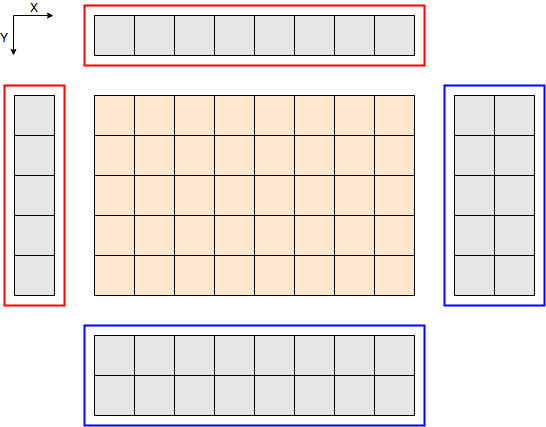
\includegraphics[width=0.9\linewidth]{2D_Block.png}
  \caption{In the middle and in light red the grid points belonging to this subdivision.
Outside in gray the four halo regions.
The red and blue lines surrounding the halo region indicates negative and positive directions respectively.}
  \label{fig:2DBlock}
\end{subfigure}%
\begin{subfigure}{0.2\textwidth}
  \centering
  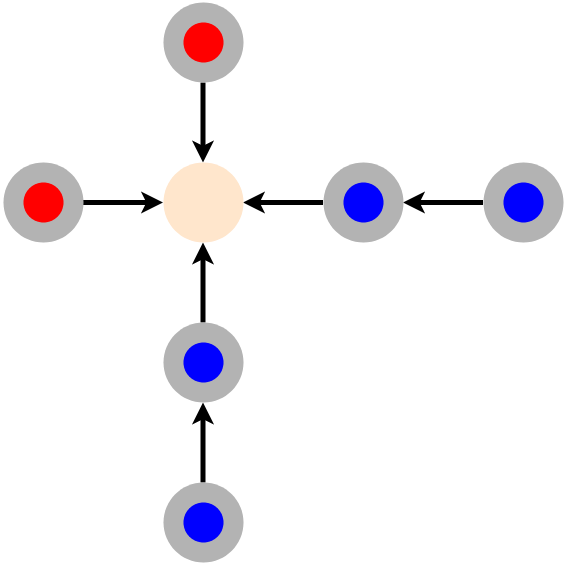
\includegraphics[width=0.9\linewidth]{2D_Block_stencil.png}
  \caption{Stencil representation corresponding to the subdivision on the left panel.}
  \label{fig:2DBlockStencil}
\end{subfigure}
\caption{Schematic view of a single two-dimensional domain subdivision.}
\label{fig:2D_subdivision}
\end{figure}

\begin{figure}[!htbp]
\centering
\begin{subfigure}{0.8\textwidth}
  \centering
  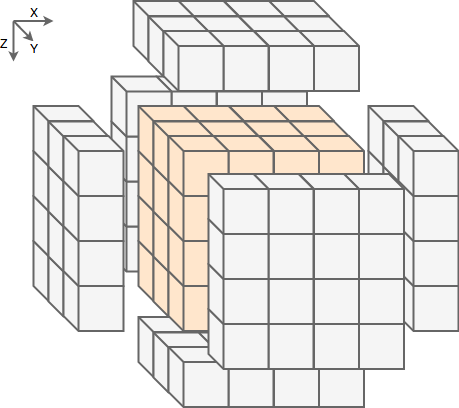
\includegraphics[width=0.9\linewidth]{3D_Block.png}
  \caption{In the middle and in light red the grid points belonging to this subdivision.
Outside in gray the six halo regions.}
  \label{fig:3DBlock}
\end{subfigure}%
\begin{subfigure}{0.2\textwidth}
  \centering
  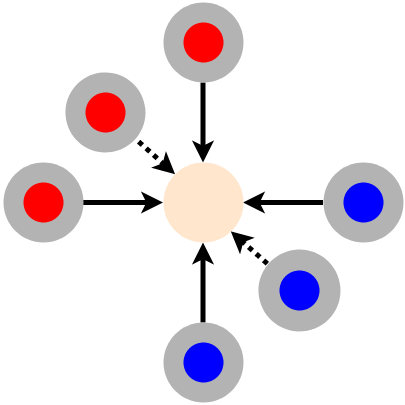
\includegraphics[width=0.9\linewidth]{3D_Block_stencil.png}
  \caption{Stencil representation corresponding to the subdivision in figure \ref{fig:3DBlock}.}
  \label{fig:3DBlockStencil}
\end{subfigure}
\caption{Schematic view of a single three-dimensional domain subdivision.}
\label{fig:3D_subdivision}
\end{figure}

\subsubsection{Source graph generation}
\label{sec:sourcegraphgeneration}
With the subdivision model definition and the two cost functions defined the source graph can be easily generated.
As shown in lines 14 to 20 of Algorithm \ref{alg:domaindecomposition} the source graph is generated as a weighted adjacency list by iterating over all subdivisions to determine their neighbors and handle the physical domain boundaries.

Determining the neighbors is an uncomplicated index calculation, as shown in Eq. \ref{eq:index} and handling the physical domain boundaries only requires catching the corresponding cases during the index calculation.

\begin{equation}
neighborindex = \left(\left(i + x\right) \cdot ndy + \left(j + y\right)\right) \cdot ndz + \left(k + z\right) \text{ ,}
\label{eq:index}
\end{equation}
where $i, j, k$ are the index number of the current subdivision in each dimension, and $x, y, z$ are either $-1$ for the negative neighbor in the corresponding direction, $+1$ for the positive neighbor in the direction, and $0$ otherwise. 
Also, $ndy, ndz$ are the number of subdivisions in y-direction and z-direction respectively.

The weighted adjacency list consists of four arrays.
The array $vweights$ contains the vertex weight for each subdivision i.e. vertex, thus its length is equal to the total number of subdivisions.
The array $eweights$ similarly contains the edge weight for each edge, and is therefore twice as long as the number of edges.
The array $adjncy$ contains the index of the end vertex for each edge, and is therefore twice as long as the number of edges.
The order in $adjcny$ determines the starting vertex for each edge.
It starts with the edges of the vertex with index 0, after all edges of vertex 0 it continues with edges of vertex 1 and so on.
And lastly the array $xadj$ contains for each vertex the $adjncy$-index for the first edge that does not belong to the vertex.
The array $xadj$ has the length of the total number of subdivisions.

The two arrays containing information about the edges are twice as long as the number of edges since graph partitioning methods do not require undirected graphs, even though for domain decomposition only undirected graphs are used.

An example adjacency list in this format can be seen in fig. \ref{fig:adjacency}, this adjacency list is the one corresponding to the source graph used in fig. \ref{fig:sourcegraph}.

\begin{figure}[!htbp]
  \centering
  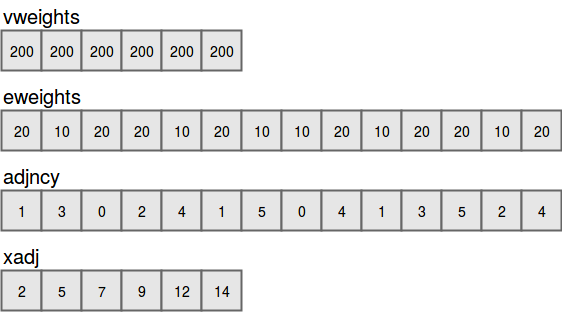
\includegraphics[width=0.8\linewidth]{adjacency.png}
  \caption{Weighted adjacency list arrays for source graph in the left panel.}
  \label{fig:adjacency}
\end{figure}

\subsection{Load balancing - graph partitioning method}
Once a domain is over-decomposed and the model has used its communication and computational cost estimates to generate a source graph the graph partitioning algorithm can be used to distribute the subdivisions into one partition for each processing unit.

Graph partitioning on such a weighted source graph means cutting the graph into partitions such that the edge cut between all partitions is minimized (i.e. minimal communication cost) while also keeping the vertex weights balanced (e.g. balanced computational cost).

More details about the graph partitioning method can be found in \citet{karypis1998multilevel} and are not the focus of this thesis.

The output of the graph partitioning methods is a list of indices for each vertex i.e. subdivision the index corresponds to a partition i.e. the index of a processing unit.

\paragraph{A small example}to demonstrate a few of the key characteristics of graph partitioning is shown in Fig. \ref{fig:sourcegraph}.
Specifically, Fig. \ref{fig:sourcegraph} shows three possible partitions for an example source graph.
For visual simplicity a two-dimensional domain is used, however a three-dimensional domain would work in the same way.
The source graph corresponds to a domain of size $30 \times 40$ with three subdivisions in x-direction and two subdivisions in y-direction.
In this example these six subdivisions are partitioned into two partitions, represented by the color of the circle in the Fig. \ref{fig:cut1}, Fig. \ref{fig:cut2}, and Fig. \ref{fig:cut3}.

Figure \ref{fig:cut1} shows a case where a graph partitioning cut causes a computational imbalance between the partitions.
Partitioning one subdivision more to one partition in such a small example causes a very large imbalance.
Usually the graph partitioning method would not allow a result with this much imbalance.
However, in larger graphs some computational imbalance up to a threshold is very common.
Most graph partitioning methods allow manipulating the imbalance threshold.

The mixed direction cut shown in Fig. \ref{fig:cut2} has the largest communication cost of the three partitions shown here.
However, it is a fully valid partition and partition boundaries that look similar are common in partitioning of larger graphs.
See the boundary between the brown and red partition in Fig. \ref{fig:metis1} for example.
This should highlight the importance of having defined clear and simple defined boundaries in the subdivision model, since the graph partitioning model already adds complexity to the partition boundaries.

Finally, Fig. \ref{fig:cut3} shows the ideal case for this small example.
Ideal cuts like this are only likely in such small and simple cases.

\begin{figure}[!htbp]
\centering
\begin{subfigure}{0.43\textwidth}
  \centering
  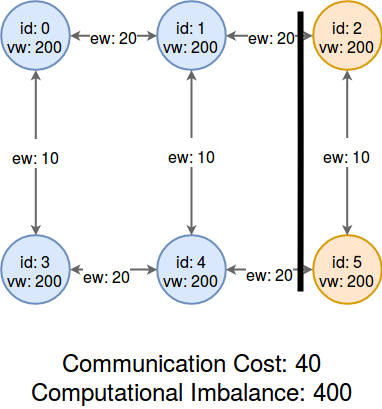
\includegraphics[width=0.95\linewidth]{source_graph_cut3.png}
  \caption{X-direction cut.}
  \label{fig:cut1}
\end{subfigure}%

\begin{subfigure}{0.43\textwidth}
  \centering
  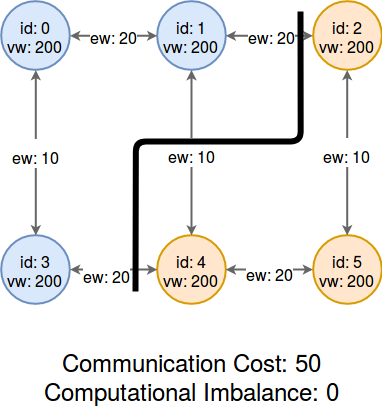
\includegraphics[width=0.95\linewidth]{source_graph_cut2.png}
  \caption{Mixed direction cut.}
  \label{fig:cut2}
\end{subfigure}%

\begin{subfigure}{0.43\textwidth}
  \centering
  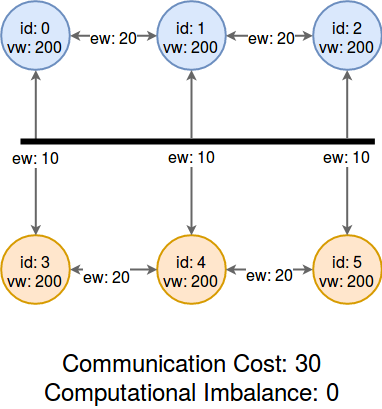
\includegraphics[width=0.95\linewidth]{source_graph_cut1.png}
  \caption{Y-direction cut.}
  \label{fig:cut3}
\end{subfigure}\hfill
\caption{Visual representation for a small graph partitioning example.
Each circle represents one subdivision of size $10 \times 20$.
The label "id" is the subdivision identification number.
The label "vw" describes the vertex weight and is equal to the size of the subdivision.
The label "ew" describes the edge weight and is equal to the size of the boundary between the corresponding subdivisions.
The color of the circle depicts the corresponding partition.
The thick, black line shows the boundary between the two partitions i.e. the cut chosen by the graph partitioning.}
\label{fig:sourcegraph}
\end{figure}

\subsection{Example subdivision and domain decomposition}
\label{sec:examplesubdivision}
The following example should highlight some aspects of the discussed subdivision and domain decomposition.

All the following figures in this section use the same domain and stencil.
The domain has size $2048 \times 1024 \times 40$ and the stencil extents are given as $\left[1, 1, 1, 1, 0, 0\right]$.
This means the stencil uses $1$ neighboring grid point in negative and positive x- and y-direction.
The boundary of the domain is also periodic in x-direction and non-periodic in y- and z- direction.

Figures \ref{fig:metis1}, \ref{fig:pymetis1}, and \ref{fig:scotch1} show the results if the domain is split into $16 \times 8 \times 1$ subdivisions.
This means every box in the figures represents $128 \times 128 \times 40$ grid points.

For comparison Figs. \ref{fig:metis2}, \ref{fig:pymetis2}, and \ref{fig:scotch2} show the results if the domain is split into $32 \times 16 \times 1$ subdivisions.
This means every box in the figures represents $32 \times 32 \times 40$ grid points and 4 of these boxes correspond to one box in the figures on the left side.

This comparison should highlight the difference the number of subdivisions and their size can make for the overall domain decomposition.
Also the difference the graph partitioning can make is shown in Fig. \ref{fig:rectangular1}.


\begin{figure}[!htbp]
\centering
\begin{subfigure}{0.5\textwidth}
  \centering
  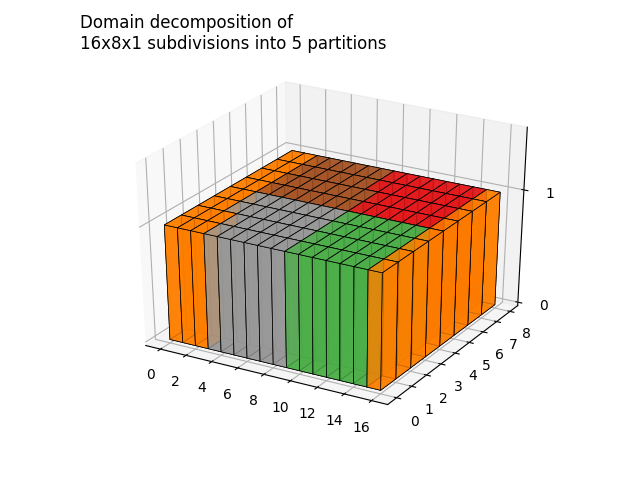
\includegraphics[width=0.9\linewidth]{metis16Px8x1.png}
  \caption{Partitioned by Metis.}
  \label{fig:metis1}
\end{subfigure}%
\begin{subfigure}{0.5\textwidth}
  \centering
  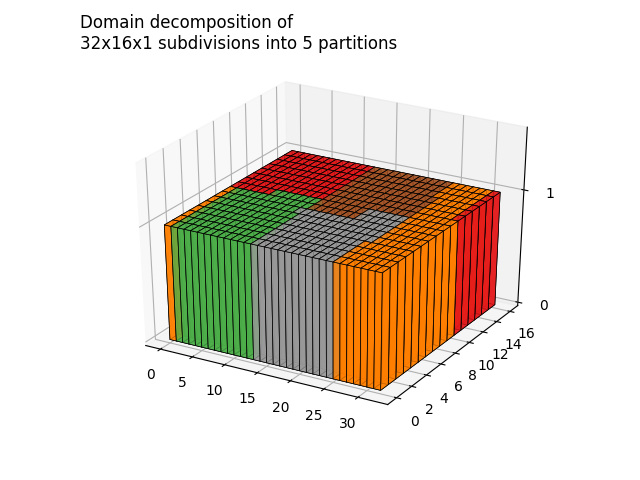
\includegraphics[width=0.9\linewidth]{metis32Px16x1.png}
  \caption{Partitioned by Metis.}
  \label{fig:metis2}
\end{subfigure}

\begin{subfigure}{0.5\textwidth}
  \centering
  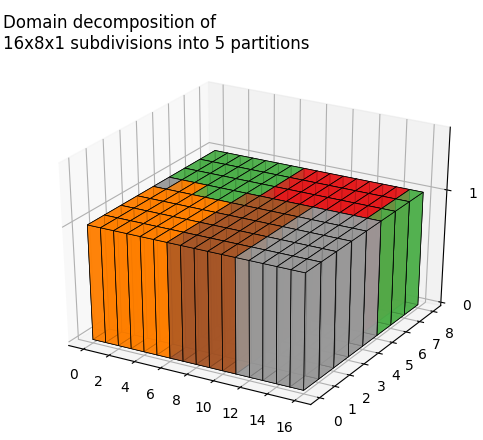
\includegraphics[width=0.9\linewidth]{pymetis16Px8x1.png}
  \caption{Partitioned by PyMetis}
  \label{fig:pymetis1}
\end{subfigure}%
\begin{subfigure}{0.5\textwidth}
  \centering
  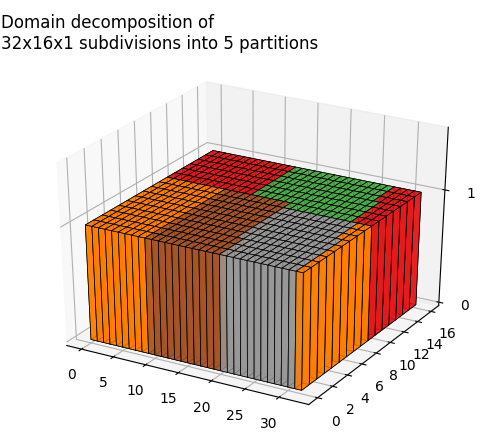
\includegraphics[width=0.9\linewidth]{pymetis32Px16x1.png}
  \caption{Partitioned by PyMetis}
  \label{fig:pymetis2}
\end{subfigure}

\begin{subfigure}{0.5\textwidth}
  \centering
  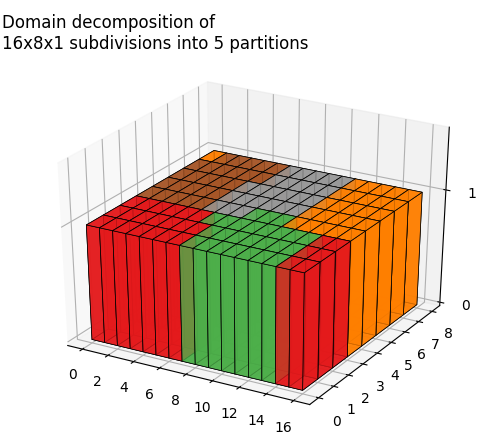
\includegraphics[width=0.9\linewidth]{scotch16Px8x1.png}
  \caption{Partitioned by Scotch}
  \label{fig:scotch1}
\end{subfigure}%
\begin{subfigure}{0.5\textwidth}
  \centering
  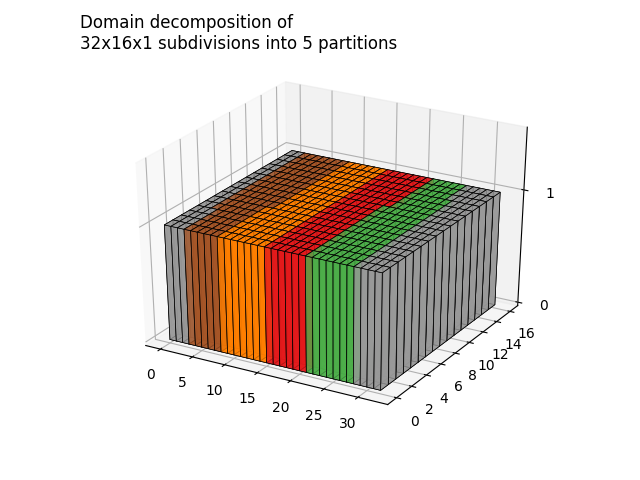
\includegraphics[width=0.9\linewidth]{scotch32Px16x1.png}
  \caption{Partitioned by Scotch}
  \label{fig:scotch2}
\end{subfigure}

\caption{Domain subdivision and domain decomposition into 5 partitions. 
Each box represents one subdivision of grid points.
Each color represents one partition. 
The domain has size 2048 x 1024 x 40 and a periodic boundary in x-direction.
Even though the domain is fully three dimensional, the domain is only decomposed in the x-y plane i.e. the horizontal plane.
Such a decomposition represents an often encountered use case for domains where the size of the two horizontal dimensions are much larger than the size of the vertical dimension e.g. numerical weather prediction models.
Not decomposing in the vertical dimension is important for locality and performance since the vertical dimension is usually the innermost loop dimension.
This also fits with many parameterizations that use the single column model assumption.
}
\label{fig:rectangular1}
\end{figure}

